\documentclass[a4paper,11pt]{article}
\usepackage[utf8]{inputenc}
\usepackage{algorithmic}
\usepackage{algorithm}
\usepackage{pst-plot}
\usepackage{graphicx}
\usepackage{endnotes}
\usepackage{graphics}
\usepackage{floatflt}
\usepackage{wrapfig}
\usepackage{amsfonts}
\usepackage{amsmath}
\usepackage{verbatim}
\usepackage{hyperref}
\usepackage{multirow}
\usepackage{pdflscape}

\usepackage{hyperref}
\hypersetup{pdfborder={0 0 0 0}}

\pdfpagewidth 210mm
\pdfpageheight 297mm 
\setlength\topmargin{0mm}
\setlength\headheight{0mm}
\setlength\headsep{0mm}
\setlength\textheight{250mm}	
\setlength\textwidth{159.2mm}
\setlength\oddsidemargin{0mm}
\setlength\evensidemargin{0mm}
\setlength\parindent{7mm}
\setlength\parskip{0mm}

\newenvironment{exercise}[3]{\paragraph{Exercise #1: #2 (#3pt)}\ \\}{
\medskip}
\newcommand{\question}[2]{\setlength\parindent{0mm}\ \\$\mathbf{Q_#1:}$ #2\ \\}

\author{\large{Ilya Kuzovkin, Raul Vicente}}
\title{\huge{Introduction to Computational Neuroscience}\\\LARGE{Practice II: Data Analysis - Continuous Data}}

\begin{document}
\maketitle

\begin{exercise}{1}{Discrete Fourier Transform (DFT)}{0.5}
Fourier transform is possible because, as it turned out, any function can be represented as a sum of sinusoidal functions (with different frequencies and amplitudes). If you have some variable changing over time you can transform this data from \emph{time domain} (time on one axis and value of the variable on the other) to \emph{frequency domain} (frequency on one axis and it's \emph{power} on the other) to see if there is any periodicity in the changes of that variable.
Transformation is defined both for continuous and discrete data. The equation for the discrete one is
$$X_f = \displaystyle\sum_{t=0}^{N-1}x_t e^{-i2\pi f\frac{t}{N}}$$
where
\begin{itemize}
\itemsep 0em
	\item $f$ is the frequency of the component, contribution of which you are trying to estimate
	\item $X_f$ is a complex number, that encodes both amplitude and phase of sinusoidal component
	\item $x_t$ is a value of the variable at time point $t$
	\item $N$ is the total number of time points
\end{itemize}
The following formula is used to extract amplitude from the complex number $X_f$:
$$A_f = \frac{\sqrt{\text{Re}(X_k)^2 + \text{Im}(X_k)^2}}{N}$$
\textbf{WHY I ACTUALLY NEED TO DIVIDE BY 2N? SEE MATLAB EXAMPLE}\\
Here you see a function, which is actually a sum of three sinusoids. Your task is to apply DFT and find out frequencies and amplitudes of those components.
\begin{figure}[htbp]
   \centering
   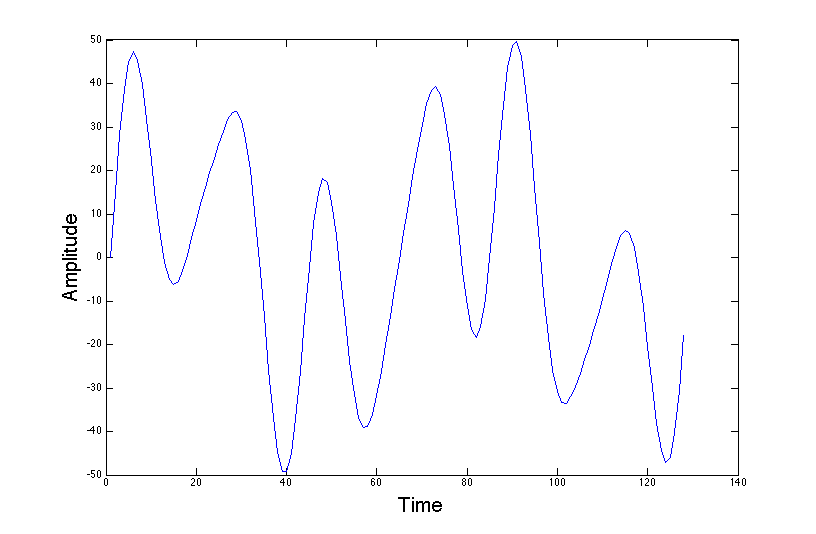
\includegraphics[width=0.4\textwidth]{dodft.png} 
\end{figure}
In the file dodft.txt you can find values for this curve.
\end{exercise}

\begin{exercise}{1}{Questionnaire}{0.5}
\question{2}{Nyquist theorem ...}
\end{exercise}

\begin{exercise}{2}{Frequency Analysis}{1}
In this exercise we ... \\
\textbf{Get data from Andero}
\begin{enumerate}
\itemsep 0em
	\item Download and study data, you have two conditions
	\item Do Fourier and plot frequency distributions for each condition
	\item What difference do you see, why?
\end{enumerate}
\end{exercise}

\begin{exercise}{3}{Correlation}{0.5}
Compute correlation between two EEG channels.
\end{exercise}

\begin{exercise}{4*}{Graph of correlations}{0.5}
blabla
\end{exercise}


\begin{exercise}{5}{Evoked Potential}{0.5}
Average over many runs to see that only then stuff becomes visible
\end{exercise}


\begin{exercise}{6}{???}{0.5}
Discuss something
\end{exercise}
\ \\
\ \\
\ \\
\ \\
\ \\
Please submit a \texttt{pdf} report with answers to the questions and comments about your solutions. Also submit a code for the programming exercise(s). Pack those into \texttt{zip} archive and upload to the course web page.

\end{document}










